\documentclass[a4paper,12pt,onsided]{article}

\usepackage[utf8]{inputenc}
\usepackage[T1]{fontenc}
\usepackage{lmodern}
\usepackage{hyperref}
\usepackage{xcolor}
\definecolor{gray}{gray}{0.50}
\definecolor{orange}{rgb}{1.0,0.5,0.0}
\definecolor{violet}{rgb}{0.6,0.0,1.0}
\definecolor{darkviolet}{rgb}{0.4,0.0,0.7}
\definecolor{darkred}{rgb}{0.8,0.2,0.2}
\definecolor{darkyellow}{rgb}{0.8,0.8,0.0}
\definecolor{darkgreen}{rgb}{0.0,0.7,0.0}
\definecolor{darkergreen}{rgb}{0.0,0.5,0.0}
\definecolor{darkcyan}{rgb}{0.0,0.7,0.7}
\definecolor{darkercyan}{rgb}{0.0,0.5,0.5}
\definecolor{lightblue}{rgb}{0.3,0.6,0.7}
\definecolor{darkblue}{rgb}{0.0,0.0,0.7}
\definecolor{darkerblue}{rgb}{0.0,0.0,0.5}
\definecolor{chocolate}{rgb}{0.8235,0.4118,0.1176}
\usepackage[left=23mm,right=23mm,top=23mm,bottom=27mm]{geometry}

\usepackage{pgfplots}[2010/07/14]

\usetikzlibrary{calc,fadings}
\usetikzlibrary{arrows}
\usetikzlibrary{arrows.meta}
\usepgfmodule{shapes}
\usepgflibrary{shapes.geometric}
\pgfplotsset{compat=1.12}

\hypersetup{colorlinks,hyperindex,plainpages=false,
  pdftitle={Abstract: Design Methodology for Custom Reconfigurable Logic Architectures},
  pdfauthor={Johann Glaser},
  pdfsubject={Abstract},
  pdfkeywords={Design Methodology, Reconfigurable Logic, Ultra-Low-Power, Application Domain Specific, Coarse-Grained, Mixed-Grained},
  pdfpagelabels,
  pagebackref,
  bookmarksopen=false}

\hypersetup{colorlinks=true}
\hypersetup{linkcolor=darkerblue}
\hypersetup{anchorcolor=black}
\hypersetup{citecolor=darkerblue}
\hypersetup{filecolor=darkerblue}
\hypersetup{menucolor=darkerblue}
\hypersetup{runcolor=filecolor}
\hypersetup{urlcolor=darkerblue}

\newcommand{\TODO}[1]{\setlength{\fboxrule}{1mm}\fcolorbox{red}{yellow}{\textcolor{blue}{TODO: #1}}}

\setlength{\parindent}{0pt}
\setlength{\parskip}{8pt}

\title{\vspace{-1mm}\sf Design Methodology for\\[2mm]Custom Reconfigurable Logic Architectures}
\date{}  % set empty --> also removes the vertical space :-)
\author{Johann Glaser}

\begin{document}
\pagestyle{empty}
\maketitle
\thispagestyle{empty} % override \maketitle's choice

\subsection*{Description}

In current trends towards ubiquitous computing and the Internet of Things (IoT), low power consumption is of
increasing concern, for example in wireless sensor network (WSN) nodes. One approach
to reduce the power consumption is to off-load the CPU by autonomous modules. These
relieve the CPU from simple tasks, e.g., performing periodic sensor
measurements. The CPU in turn stays in an inactive low-power mode for extended periods. It
is only activated if more complex tasks have to be accomplished, such as
communicating a new value
via the wireless network. Such autonomous CPU supplement modules are
implemented as logic designs. These must be reconfigurable to
maintain the flexibility for the realization of different applications, to
allow adaption to new environments, and to fix design issues. In
 \cite{Gla15} a new design methodology for the development of such reconfigurable CPU supplement
modules is introduced.

%\ifShowHidden
%The proposed design methodology has to result in functioning and verified
%reconfigurable modules which must be able to implement all specified
%functionality. These modules must consume less energy to perform the specified
%functionality, compared to the CPU. Further more, these modules must utilize
%less chip area than the parallel implementation of all planned functionality,
%and less chip area than an implementation using an embedded FPGA. Its
%configuration data must be smaller than for an embedded FPGA implementation.
%The design process must not require additional skills of chip designers and,
%together with the final reconfigurable module, must be compatible to commercial
%tools as well as in-house design flows. The reconfigurable module must be fully
%verified and it must provide additional flexibility, so that new
%functionality, not anticipated during the design process, can be implemented after production.
%\fi

% pre-si
Contrary to FPGA design, where chips with a predefined reconfigurable
architecture are configured, the proposed methodology includes the development
of the silicon circuitry itself.
% control+data
The reconfigurable modules have to support both, control-dominated tasks as
well as data processing.
% mixed-grained --> heterogeneous --> app.dom.spec.
To reduce silicon area and power consumption, the approach utilizes a
mixed-granularity logic architecture.
Besides fine-grained functional units and signals, this adds coarse-grained
functional units with more complex functionality and operating on multi-bit
vectors.
This requires that heterogeneous, i.e., multiple different kinds of functional
units, are integrated.
This further requires, that each reconfigurable module is specifically developed
for its given application domain.
% --> design methodology
The design methodology proposed in \cite{Gla15} addresses this task.

% SotA, scientific basis, scientific gap
State of the art design methodologies for reconfigurable logic architectures
are limited to application domains for data processing but do not support
cycle-accurate control-dominated tasks.
% no mixed-grained
These approaches either use coarse-grained or fine-grained architectures, but
do not provide mixed granularity reconfigurable logic.
% mapping
%The functionality of the reconfigurable logic is specified with a set of
%applications which must be supported.
The functional units of the reconfigurable logic either have to be
instantiated explicitly or are mapped manually.

The design methodology introduced in  \cite{Gla15} solves these issues.
% architecture
The underlying architecture % is defined as a collection of reconfigurable functional units
%connected via a reconfigurable interconnect and 
specifically supports mixed
granularity logic.
% specification
The functionality of reconfigurable modules is specified with a set of example
applications as VHDL or Verilog logic designs. These enable the definition of
control-dominated as well as data processing tasks including all signals and
cycle accurate timing.
% generation
From these the functional units and the interconnect are optimized in a novel
semi-automatic procedure.

% IP core
The resulting reconfigurable module is delivered as an IP core for the
integration in a chip design.
% result
It can implement any of the example applications and provides flexibility to
implement new applications which were not anticipated during the design
process.
% oversizing
In order to further increase its flexibility, additional functional units and
routing resources
can be included during the optimization.
% verification
The design methodology is the first to incorporate full verification of the example
applications, of all intermediate steps, and of the generated reconfigurable
module. Simulation and logical equivalence checking are used to ensure
compliance to the specification.
                                           
The design methodology was implemented as an EDA design flow incorporating custom,
open-source, and commercial tools.
All tasks which are not essentially manual are automated to assist the
designer and to achieve high productivity.
The design flow was used to develop an exemplary WSN node SoC including a reconfigurable
sensor interface module.
This application domain includes control-dominated tasks as well as data
processing. 
The WSN SoC was produced in a 350\,nm CMOS process. It correctly implements
all example applications and new applications.
This demonstrates the feasibility of the design methodology.
%
The reconfigurable module shows
a 180-fold reduction in energy consumption for sensor measurements, compared to
the integrated CPU.
Its chip area is
%2.2 times larger than the parallel implementation of all example and new
%applications but
4.0--4.3 times smaller and it requires 9.1--23.4 times less configuration data than
embedded FPGAs.
Additionally it provides
enough flexibility to implement diverse new applications and to fix
design issues of example applications.

To summarize, the following images classify the approach of \cite{Gla15} in terms
of flexibility, power consumption, chip area, and performance.

\vspace{5mm}

  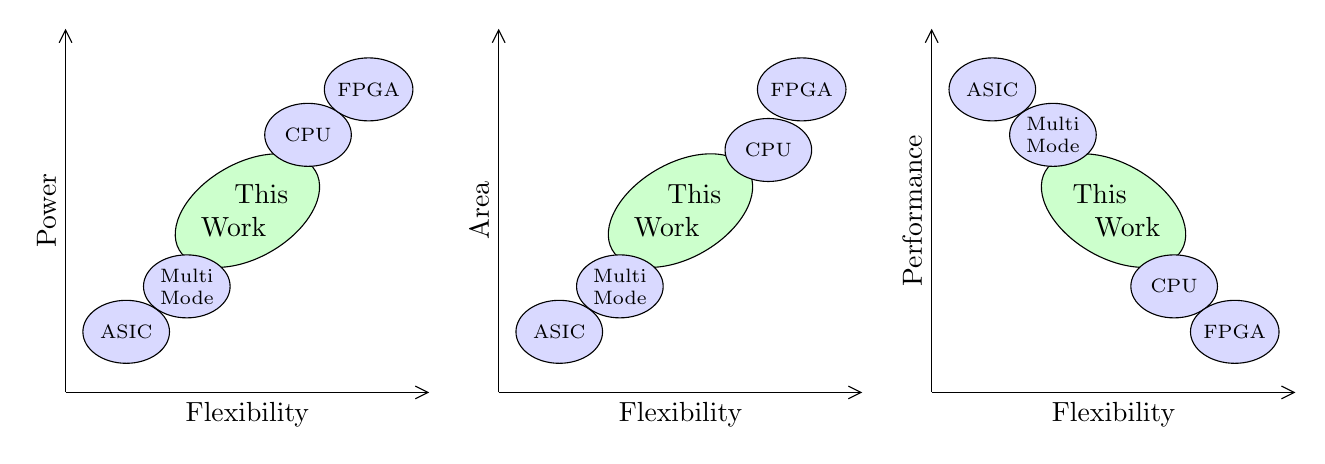
\begin{tikzpicture}[
      ell/.style={
        draw,
        ellipse,
        shape border uses incircle=true,
        align=center,
        font=\scriptsize,
        inner sep=0pt,
        minimum width=11mm,
        minimum height=8mm,
        fill=blue!15,
      },
    ]
    \begin{axis}[
        compat=newest,
        width=62mm,
        height=62mm,
        axis x line=bottom,
        axis y line=left,
        x axis line style={-{Straight Barb[scale length=2pt]}},
        y axis line style={-{Straight Barb[scale length=2pt]}},
        xlabel={Flexibility},
        ylabel={Power},
        ticks=none,
        xmin=-1, xmax=11,
        ymin=-1, ymax=11,
      ]
      \node [ell] at (1,1) {ASIC};
      \node [ell,minimum width=20mm,minimum height=12mm,rotate=30,fill=green!20] at (5,5) {};
      % "shape border rotate" doesn't work for "ellipse" :-( --> separate text :-)
      \node [align=center] at (5,5) {~~~This\\Work~~~~};
      \node [ell] at (3,2.5) {Multi\\Mode};
      \node [ell] at (7,7.5) {CPU};
      \node [ell] at (9,9) {FPGA};
    \end{axis}
    \begin{axis}[
        xshift=55mm,
        compat=newest,
        width=62mm,
        height=62mm,
        axis x line=bottom,
        axis y line=left,
        x axis line style={-{Straight Barb[scale length=2pt]}},
        y axis line style={-{Straight Barb[scale length=2pt]}},
        xlabel={Flexibility},
        ylabel={Area},
        ticks=none,
        xmin=-1, xmax=11,
        ymin=-1, ymax=11,
      ]
      \node [ell] at (1,1) {ASIC};
      \node [ell,minimum width=20mm,minimum height=12mm,rotate=30,fill=green!20] at (5,5) {};
      % "shape border rotate" doesn't work for "ellipse" :-( --> separate text :-)
      \node [align=center] at (5,5) {~~~This\\Work~~~~};
      \node [ell] at (3,2.5) {Multi\\Mode};
      \node [ell] at (7.9,7) {CPU};
      \node [ell] at (9,9) {FPGA};
    \end{axis}
    \begin{axis}[
        xshift=110mm,
        compat=newest,
        width=62mm,
        height=62mm,
        axis x line=bottom,
        axis y line=left,
        x axis line style={-{Straight Barb[scale length=2pt]}},
        y axis line style={{Straight Barb[scale length=2pt]}-},  % arrow on other side due to "y dir=reverse"
        xlabel={Flexibility},
        ylabel={Performance},
        ticks=none,
        xmin=-1, xmax=11,
        ymin=-1, ymax=11,
        y dir=reverse, % being lazy :-)
      ]
      \node [ell] at (1,1) {ASIC};
      \node [ell,minimum width=20mm,minimum height=12mm,rotate=-30,fill=green!20] at (5,5) {};
      % "shape border rotate" doesn't work for "ellipse" :-( --> separate text :-)
      \node [align=center] at (5,5) {This~~~~\\~~~Work};
      \node [ell] at (3,2.5) {Multi\\Mode};
      \node [ell] at (7,7.5) {CPU};
      \node [ell] at (9,9) {FPGA};
    \end{axis}
  \end{tikzpicture}%

\vspace{10mm}
\subsection*{Unique Contributions}
\begin{itemize}
  \item \textbf{Design Methodology.}
    The main contribution of \cite{Gla15} is a design methodology for the
    development of reconfigurable CPU supplement modules which are optimized
    for a given application domain.
    It is the first design methodology which is universal and independent of
    the application domain of the generated reconfigurable modules.
    This is achieved by the introduction of the concurrent support of both,
    control-dominated tasks and data processing.
    Previous design methodologies were limited to data processing and did not
    support cycle accurate control-dominated tasks.

    The feasibility, applicability, and correctness of the design methodology
    were demonstrated with a manufactured reconfigurable module which
    implements a WSN node sensor interface.
    The experimental results show that the design methodology leads to a
    functioning reconfigurable module which correctly implements the specified
    functionality.
    Additionally, enough flexibility is provided to implement new
    functionality. The reconfigurable module requires less power compared to a
    CPU to perform the same task.
    It requires less chip area and less configuration data than an embedded
    FPGA.

    Besides a sensor interface, the independence of the application domain and
    the universality of the design methodology enable the implementation of
    other tasks which are neither related to WSNs nor to low power consumption.
    Firstly, applications which require a given degree of flexibility benefit
    from the reduced power consumption, chip area, and size of the
    configuration data, compared to other reconfigurable or programmable
    architectures.
    Secondly, the introduced design methodology enables applications to
    include flexibility after production, which was previously precluded
    due to complexity, cost, chip area, or power consumption.

    For example, the introduced design methodology enables the implementation
    of new WSN network protocols. These can be based on frequent operations
    which were previously precluded due to too high power consumption of the
    CPU.
    Additional to the use as a low-power technique in WSN nodes, the resulting
    reconfigurable modules enable fast responses and constant latency to react
    on incoming information. With this feature, rapid and ultra-low-power
    real-time control loops can be implemented.
    In the research area of software defined radio (SDR), the introduced design
    methodology fills the gap between software implementations using digital
    signal processors (DSPs) and fine-grained reconfigurable logic
    implementations using FPGAs.

    Further applications include network protocol handlers, baseband
    processors, digital filters, CPU accelerators, computer
    vision preprocessors, gaming controllers, etc.
    However, an increased degree of flexibility leads
    to higher power consumption and chip area and lower performance.
    For a given application the tradeoff between these properties determines
    the benefit gained by the utilization of the introduced design methodology.

% TODO: unversality begründen

    The design methodology is based on RTL HDL designs and therefore
    independent of the semiconductor process.
    The development of a reconfigurable module and its integration into a chip
    design is straightforward and uncomplex.
    Therefore it is also suitable for small designs, wherever post-silicon
    flexibility is required, for example to avoid the use of an embedded or
    external FPGA, or within an FPGA if no partial reconfiguration is available
    or desired.
    Further, the results achieved with the design methodology are verified, i.e., the
    integration of reconfigurable modules is a secure design decision which
    does not cause additional risks.

    The design methodology effectively closes the gap between fixed function
    logic designs and fully flexible embedded FPGAs.

  \item \textbf{Transition-Based Reconfigurable FSM (TR-FSM).}
    The second core contribution of \cite{Gla15} is a novel architecture for
    reconfigurable FSMs, termed ``Tran\-si\-ti\-on-Based Reconfigurable FSM''
    (TR-FSM).
    The TR-FSM is used in the reconfigurable modules to efficiently implement
    control-dominated tasks.
    Its feasibility, applicability, and correctness were also demonstrated with
    the manufactured reconfigurable module.
    The TR-FSM architecture reduces the power consumption, chip area,
    configuration data, and propagation delay time compared to other
    reconfigurable architectures for FSMs, and allows straight-forward mapping
    algorithms.

    The TR-FSM is an independent design unit which can be integrated in SoC
    designs wherever an efficient reconfigurable FSM implementation is
    required.
    It is available as a VHDL RTL design with a number of generics which allow
    full customization of the silicon implementation to the requirements of
    the designer.
    Its actual functionality can be specified in various formats, from which the
    configuration data is generated by a dedicated tool. The configuration data
    is provided for convenient integration in design verification, firmware
    drivers, and in custom configuration infrastructure.
\end{itemize}

\vfill

\bibliographystyle{alpha}
\bibliography{../bibliography}

\end{document}
